\section{Schemat drabinkowy (Ladder Diagram)}
\label{sec:drabinka}

\subsection{Postać klasyczna}
Schemat drabinkowy pokazano na rysunku~\ref{fig:ladder}. Zastosowano
następujące oznaczenia:
\begin{itemize}
    \item \texttt{-{}-[\,]-{}-} – styk normalnie otwarty (NO),
    \item \texttt{-{}-[/]-{}-} – styk normalnie zamknięty (NC),
    \item \texttt{-{}-(\,)-{}-} – cewka wyjściowa,
    \item \texttt{TON} – przekaźnik czasowy opóźnionego załączenia
          (\SI{2}{\minute}), zerowany sygnałem $M$.
\end{itemize}

\begin{figure}[H]
\centering
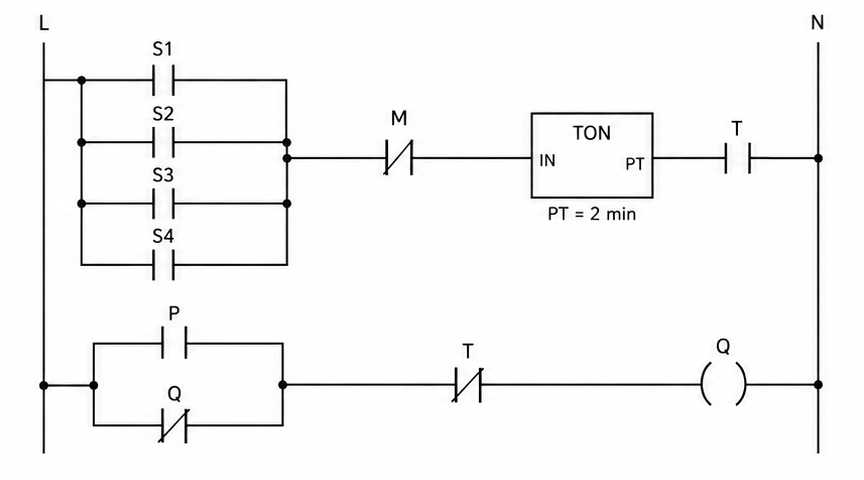
\includegraphics[width=\textwidth]{figures/Drabinkowy.png}
\caption{Schemat drabinkowy sterowania oświetleniem.}
\label{fig:ladder}
\end{figure}

\subsection{Odwzorowanie w programie LOGO!Soft Comfort}
Schemat drabinkowy został odwzorowany w programie LOGO!Soft Comfort na rysunku~\ref{fig:logo_bez_zbocza}. Pierwotnie przyjęto odrobinę błędne założenie, mianowicie nie wzięto pod uwagę faktu, że konieczne będzie użycie dodatkowego bloku wykrywania zbocza (\texttt{AND (edge) - zbocze narastające}). Brak tego bloku spowodował, że wyjście Q1 migotało ze względu na cykliczny charakter pracy sterownika PLC. Podczas przytrzymania przycisku sygnał wejściowy pozostawał w stanie wysokim przez wiele cykli programu, co w połączeniu z logiką XOR powodowało naprzemienne, błyskawiczne załączanie i wyłączanie cewki Q1.

\begin{figure}[H]
\centering
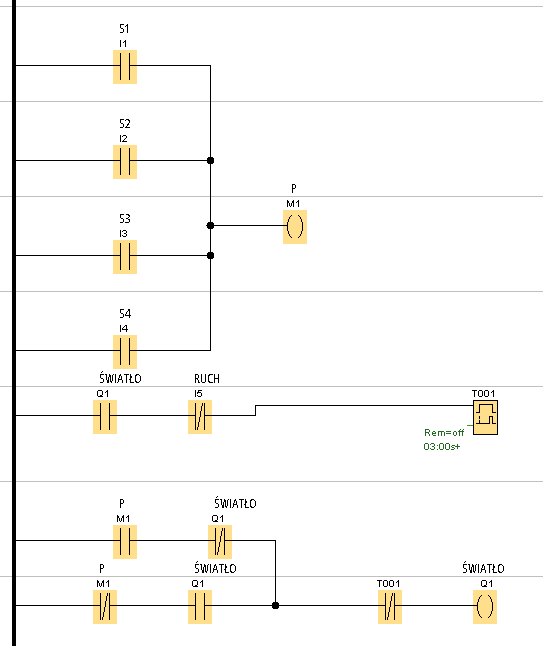
\includegraphics[width=\textwidth]{figures/logo_bez_zbocza.png}
\caption{Schemat drabinkowy odwzorowany w programie LOGO!Soft Comfort.}
\label{fig:logo_bez_zbocza}
\end{figure}

Zastosowanie bloku detekcji zbocza narastającego (SF002) całkowicie rozwiązało ten problem. Zamienia on ciągły sygnał z przycisków na pojedynczy impuls trwający dokładnie jeden cykl programu. Dzięki temu każde fizyczne naciśnięcie przycisku zmienia stan oświetlenia dokładnie raz, co zapewnia stabilną pracę układu. Dodatkowo, prawidłowe wpięcie wyjścia timera (jako styku NC w szeregu z cewką) gwarantuje, że po upływie 2 minut bezruchu światło zostanie asynchronicznie wygaszone, a układ będzie od razu gotowy na przyjęcie kolejnego impulsu z przycisków, bez konieczności resetowania stanów pośrednich. Ostateczna implementacja w pełni odzwierciedla zależność logiczną z równania \eqref{eq:rownanie_stanu} i spełnia wszystkie założenia projektowe.


\begin{figure}[H]
\centering
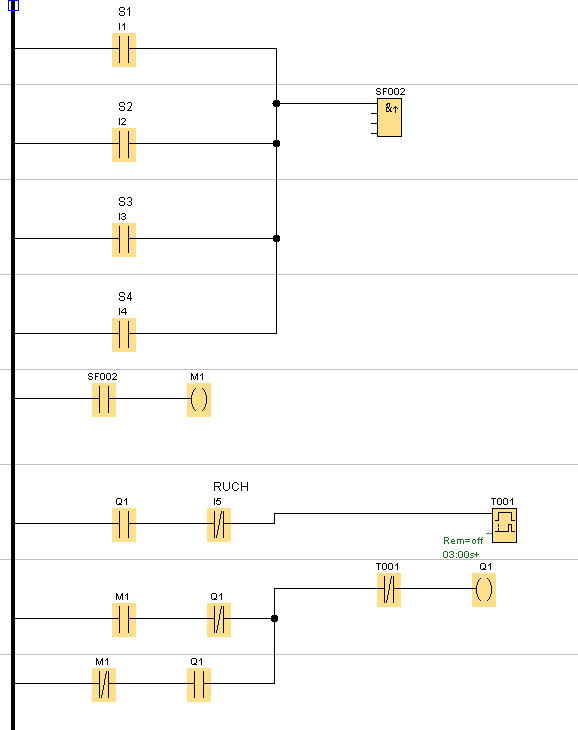
\includegraphics[width=\textwidth]{figures/logo_z_zboczem.png}
\caption{Schemat drabinkowy odwzorowany w programie LOGO!Soft Comfort z użyciem bloku detekcji zbocza narastającego (SF002).}
\label{fig:logo_z_zboczem}
\end{figure}